\documentclass{beamer}

\usepackage[frenchb]{babel}
\usepackage[T1]{fontenc}
\usepackage[utf8]{inputenc}
\usepackage{tikz}
\usetikzlibrary{quotes,angles,calc,intersections,babel,through,backgrounds,angles,positioning}
\usepackage{rotating}

\usetheme{Warsaw}

\title{Soutenance bibliographique}
\author{BESSENG A IREH Guy Raymond}
\institute[]{Université Paul Sabatier}
\date{21 Mars 2018}
\setbeamertemplate{caption}{\raggedright\insertcaption\par}
\addtobeamertemplate{navigation symbols}{}{%
    \usebeamerfont{footline}%
    \usebeamercolor[fg]{footline}%
    \hspace{1em}%
    \insertframenumber/\inserttotalframenumber
}
\begin{document}

\maketitle
\section{introduction}
\begin{frame}
\frametitle{Article}
\begin{center}
Shape and motion of drops sliding down an inclined plane

By NOLWENN LE GRAND, ADRIAN DAERR AND LAURENT LIMAT
\end{center}
\end{frame}

\begin{frame}
\frametitle{Dispositif expérimental}
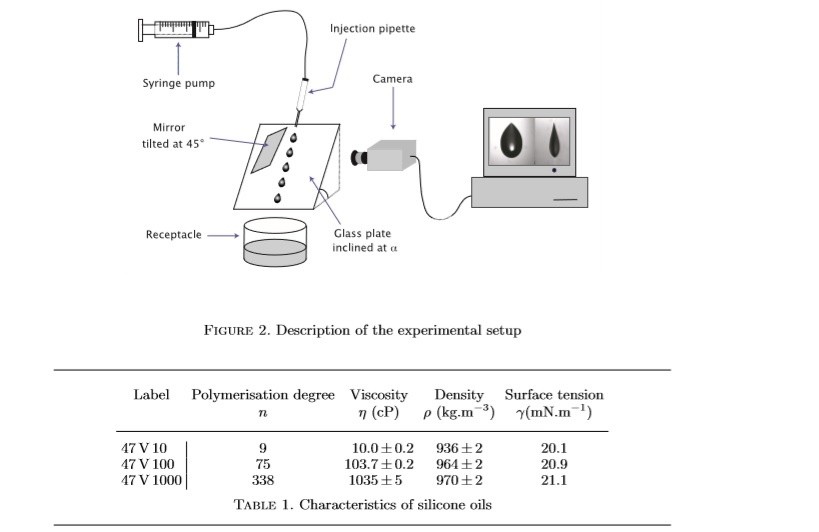
\includegraphics[scale = 0.5]{Experiment.jpg}
\end{frame}

\begin{frame}
\frametitle{Condition de mouillage}
\begin{itemize}
\item Fluoropolymère FC-725 
\item volume de la goutte : $V = (6.0 \pm 0.2) mm^{3}$
\item l'angle dynamique : $\theta_{r} < \theta < \theta_{a}$
\item $50^{\circ} < \theta < 55^{\circ}$
\end{itemize}
\end{frame}

\begin{frame}
\frametitle{Différents régimes}
\begin{center}
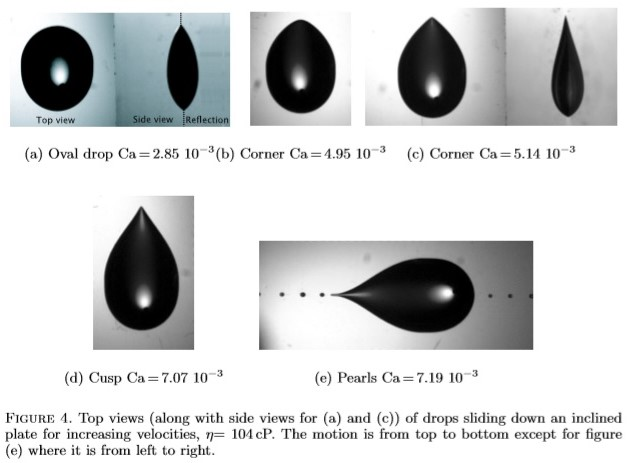
\includegraphics[scale = 0.5]{ovale_pointue.jpg}
\end{center}
\end{frame}

\begin{frame}
\frametitle{Bilan des forces}

\begin{figure}[t]
\centering
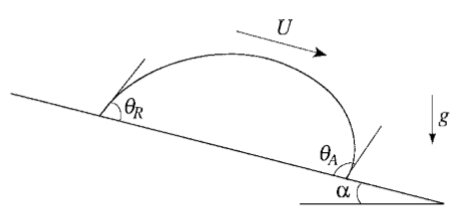
\includegraphics[scale = 0.3]{Bilan.png}
\end{figure}
\begin{itemize}
	\item Le poids : $\rho g V \sin \alpha$
	\item la force de frottement: $\eta U V^{1/3}$
	\item la tension de surface : $\gamma \Delta \theta = \gamma w \left( \cos (\theta_{R}) - \cos (\theta_{A}) \right)$
\end{itemize}
\end{frame}

\begin{frame}
\frametitle{Debut du glissement}
\begin{itemize}
\item on a glissement pour $\alpha_{c} < \alpha$
\item Pas de frottement à la limite du glissement donc $\rho g V \sin \alpha = \gamma V^{1/3} \left( \cos (\theta_{R}) - \cos (\theta_{A} ) \right)$
\item $V^{2/3}(\rho g / \gamma) \sin \alpha \simeq  \cos (\theta_{R}) - \cos (\theta_{A} ) $
\item le nombre de Bond : $B_{O} = \frac{\text{effets gravitaires}}{\text{effets inertiels}} = V^{2/3} (\rho g / \gamma)\sin \alpha$
\item $B_{O_{c}} = V^{2/3}(\rho g / \gamma)\sin \alpha_{c} = \cos (\theta_{R}) - \cos (\theta_{A} )$
\item $B_{O_{c}} = \left(\frac{24}{\pi}\right) ^{2/3} 
	\frac{\left(\cos (\theta_{R}) - \cos (\theta_{A})\right) \left(1 + \cos (\theta_{A})\right) ^{1/2}}
		{\left(2 + \cos (\theta_{A})\right) ^{1/3}\left(1 - \cos (\theta_{A})\right) ^{1/6}}$
\end{itemize}
\end{frame}


\begin{frame}
\frametitle{Gouttes en mouvement}
\begin{itemize}
\item $U$ vitesse de la goutte, $\theta(U)$?
\item Le nombre capillaire : $C_{a} = \frac{\text{effets visqueux}}{\text{effets capillaire}} = \frac{\eta U}{\gamma}$
\item De Gennes : $ \theta \left(\theta^{2} - \theta_{s}^{2}\right) = \pm 6\ln\left(\frac{b}{a}\right)C_{a}$
\item Cox et Voinov : $\theta^{3} - \theta_{s}^{3} = \pm 9\ln\left(\frac{b}{a}\right) C_{a}$
\item Cinétique moléculaire: $\left(\theta^{2} - \theta_{s}^{2}\right) = \frac{\nu NkT}{2\pi fL_{m}h}C_{a}$
\item Linéaire : $\theta - \theta_{s} \propto \pm U$
\end{itemize}
\end{frame}



\begin{frame}
\frametitle{Comparaisons avec des modèles}
\centering
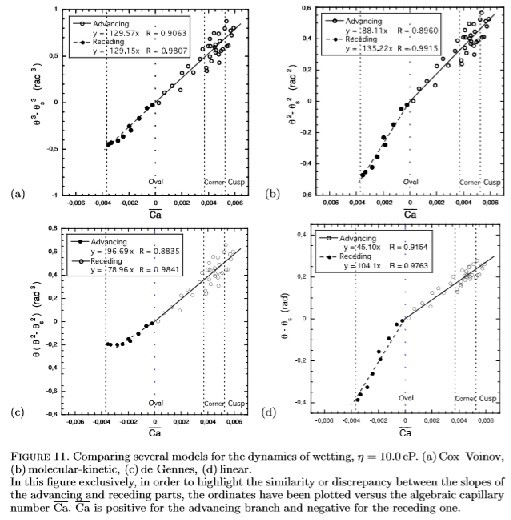
\includegraphics[scale = 0.5]{Modeles.jpg}
\end{frame}


\begin{frame}
\frametitle{Transitions entre régime}
\centering
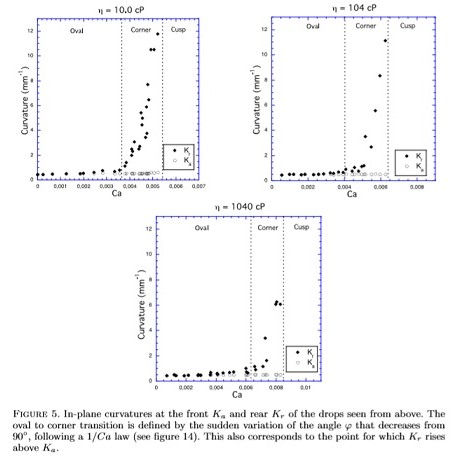
\includegraphics[scale = 0.6]{Transition.jpg}
\end{frame}


\begin{frame}
 \frametitle{goutte en coin}
\begin{figure}[t]
\centering
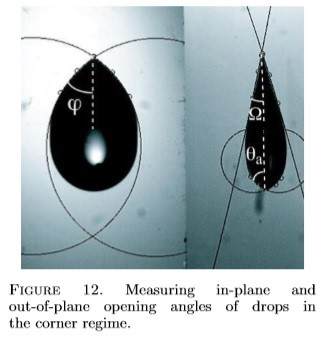
\includegraphics[scale = 0.5]{Coin.jpg}
	\caption{$\sin \varphi = \frac{\theta_{s}^{3}}{9\ln\left( \frac{b}{a} \right) C_{a}} \propto \frac{1}{C_{a}}$}
\end{figure}
\end{frame}

\begin{frame}
 \frametitle{goutte en coin}
\begin{figure}[t]
\centering
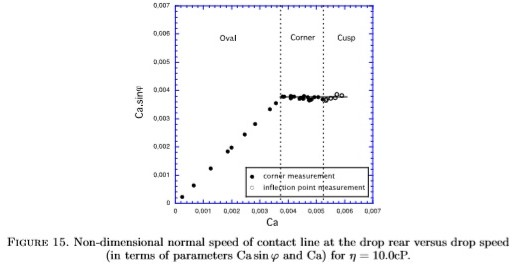
\includegraphics[scale = 0.5]{sinvarphi.jpg}
\end{figure}
\end{frame}


\begin{frame}
 \frametitle{goutte en coin}
\begin{figure}[t]
\includegraphics[scale = 0.5]{goutellette.jpg}
\centering

\end{figure}
\end{frame}

\begin{frame}
\frametitle{Conclusion}
\begin{itemize}
\item Dispositif expérimental
\item Debut de glissement à $\alpha_{c}$
\item $C_{a}$ a le même ordre de lors du changement de régime pour différente viscosité
\item Le modèle de Cox - Voinov a été utlisé pour déterminer les angle $\varphi$ et $\Omega$
\item L'émission des gouttelettes commence quand $\Omega$ prend ses valeurs les plus faibles (proche de zero)
\end{itemize}
\end{frame}

\begin{frame}
\frametitle{Rapport avec le stage}


\begin{figure}
\begin{center}
\begin{tikzpicture}[scale = 0.5]
\coordinate (0) at (0,0);
\coordinate (A) at (-10,0);
\coordinate (B) at (3,0);
\draw[color = blue] (0) arc (30:150:4) -- cycle;
\draw (A) -- (B);
\draw[<-] (0,1) -- (2,1);
\draw[<-] (-9,1) -- (-7,1);
\node[above] at (1,1) {$U$};
\node[above] (V) at (-8,1) {$F_{D}$};
\end{tikzpicture}
\end{center}
\end{figure}

\begin{figure}
\begin{center}
\begin{tikzpicture}[scale = 0.5]
\coordinate (0) at (0,0);
\coordinate (A) at (210:10);
\coordinate (B) at (30:3);
\coordinate (C) at ($ (A) + (13,0) $);
\coordinate (D) at ($(210:4)+(0,1)$);
\coordinate (E) at ($ (D) + (0,-3) $);
\draw[color = blue] (0) arc (30:210:4) -- cycle;
\draw (A) -- (B);
\draw (A) -- (C);
\draw[->] (D) -- (E);
\node[left] at (E) {$P$};
\end{tikzpicture}
\end{center}
\end{figure}
\end{frame}

\begin{frame}
\frametitle{Questions}
  \center{Avez-vous des questions ?}
\end{frame}



\end{document}
